\documentclass[11pt, a4paper]{article}
\usepackage{amsmath}
\usepackage[utf8]{inputenc}
\usepackage{amsfonts}
\usepackage{amssymb}
\usepackage{tikz}
\usepackage{array}
\usepackage{cancel}
\usepackage{ulem}
\usepackage{graphicx}
\usepackage[a4paper]{geometry}
\usepackage{gauss}
\usepackage{amsmath}
\usepackage{lastpage}
\usepackage{fancyhdr}
\usepackage{multirow}
\usepackage{listings}
\setlength{\headheight}{15.2pt}
\pagestyle{fancy}
\fancyhf{}
\lhead{Mads Anthony, MANA} %husk denne
\rhead{Side\ \thepage\ af\ \pageref{LastPage}} %husk 2 builds for dette!
\usepackage{enumerate}
\usetikzlibrary{shapes}
\begin{document}
\author{Mads Anthony}
\section{Experiments}
\subsection{Setup}
With the background knowledge of neural oscillations and their possibly important role in doing modular tasks, it could be interesting to see how new methods that use these observations perform against other successful modular methods.
\\
\\
In this section I therefore introduce two new methods that is based on neural oscillations, MiO-HyperNEAT and MaO-HyperNEAT which is explained in the beginning of this sections. The results will then be compared to two MB-HyperNeat modular methods by Schrum[ref].
\subsubsection{Microscopic Oscilliations HyperNEAT (MiO-HyperNEAT)}
The general idea with this method is to try and mimic the oscillations that happens on the microscopic level of the brain and use it to modularize the network. As mentioned earlier, the microscopic oscillations (MiO) is the firing patterns that take place for each neuron. To mimic this, MiO-HyperNEAT uses HyperNEAT together with SUPG to evolve oscillations for each hidden neuron placed on the substrate.
\\
\\
Along with the oscillation evolved for each hidden neuron the network on the substrate has an extra output that generate a \textit{Master Frequency}. The master frequency, isn't evolved using a SUPG, but is instead generated as a normal output (that if necessary can be modulated onto some pre-defined function - ex. sine function). The idea with the master frequency is to generate a frequency that is dependent on the environment, whereas the neuron oscillations only are determined by their position on the substrate.
\\
\\
Each hidden neuron then compare their oscillations with the master frequency, and if they are in synchrony they are enabled, and if not - they are disabled. One reason for this, is to let Hyper-NEAT try to discover frequencies that make part of the network be active at different times. Another reasons is that research (as mentioned earlier) points to certain oscillations be in synchrony for different task.
\\
\\
Since the total number of ways the hidden neurons can be active/disabled is $ 2^n $ it could in theory mean that Hyper-NEAT could discover $ 2^n $ modules - where $ n $ is the number of hidden neurons. A setup of the method can be seen in figure (x).
\begin{figure}[!ht]
\centering
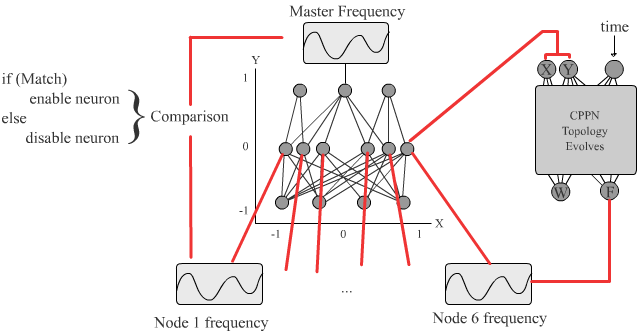
\includegraphics[scale=0.5]{MiO-HyperNEAT}
\caption{}
\end{figure}
\\
\subsubsection{MaO-HyperNEAT}
-
\subsubsection{Modifying the master frequency}
An important part of MiO-HyperNEAT is its ability to generate a master frequency. The idea for the master frequency is that it should produce some frequency that is unique for each task. What these frequency looks like is not really important, as long as the SUPG's are able to generate frequencies that matches them.
\\
\\
However, this approach makes the assumption that the master frequency is able to generate some underlying temporal structure that is unique for each task. Although this would be ideal, it might not always be the case. So to account for this, I introduce some modifications to the master frequency. These modifications are used as an alternative to the original MiO-HyperNEAT method, and are introduced to rule out problems that could exist using the master frequency. This is done by enhancing the temporal structure in the master frequency.
\\
\\
To enhance the temporal structure in the master frequency I choose to modulate the substrate output onto a carrier wave by using frequency- or amplitude modulation (FM/AM). I then define the carrier wave as  a sine wave $ sin(2 \cdot \pi \cdot x) $ and use the substrate output to change the frequency/amplitude of the carrier wave, as shown in figure (x).
\\
\\
With the use of FM modification, you could imagine the master frequency oscillating at a lower (alpha) frequency during one task and at a higher (beta) frequency during another task. This further strengthen the analogy to the previous research [ref].
\begin{figure}[!ht]
\centering
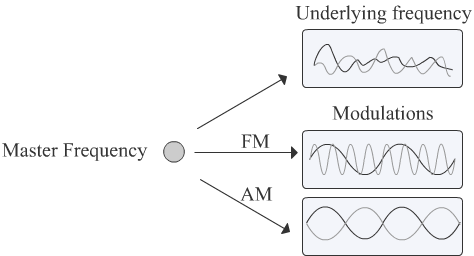
\includegraphics[scale=0.4]{Images/MasterFrequencyModulation}
\caption{}
\end{figure}
\subsubsection{Comparing SUPG frequencies with Master Frequency}
Another important part of MiO-HyperNEAT is the comparison that take place between the SUPG frequencies and the Master frequency. It seems likely that picking the right comparison measure is vital for MiO-HyperNEAET to succeed. Therefore I will in the following presents some methods that could be used to compare frequencies, and argue for my choice of comparison.
\\
\\
One simple comparison measure is to use the latest signal value from both frequencies and only enable the hidden neuron if they both lie within a certain threshold.
\subsection{Experiment 1 - Recognizing oscillations}
Before testing how the new methods perform at  multitasking, I first want to focus on the SUPG part and test how good it is at recognizing oscillations. To do this I give it a sample of predetermined functions that the SUPG then has to try and replicate.
\\
\\
Recall that the SUPG takes the neuron's position on the substrate along with a timer. The timer is increased by 1 on each tick, and the maximum value is determined by the wavelength. I set the wavelength to 100 and divide the timer by the wavelength - so that the input to the SUPG span 0 to 1. Since the SUPG will repeat itself after one cycle, it's unnecessary to evaluate more than one cycle. So I let each genome timeout after 100 ticks.
\\
\\
To compare two functions I use the sum of squares, which takes the squared distance for each point and sum it together. I then define the fitness function in the following way, where $ y_i $ is the original function values and $ y_i' $ is the values generated by the SUPG.
\begin{equation} F = 1 - \dfrac{\sum_{i=0}^{100}(y_i-y_i^{'})^2}{100} \end{equation}
Notice that to maximize the fitness function you have to minimize the sum of squares and that the maximum fitness value is 1. Also since the SUPG only encodes values from 0 to 1 the predetermined functions that the SUPG has to recognize will have to exist in this span as well.
\\
\\
To generate matching oscillations the SUPG has to evolve it's topology using NEAT. Recall that for each new added node, a random activation function is chosen. The list of activation functions I used was the following: bipolar-sigmoid, sine, linear and gaussian. All these was chosen from an even distribution. Although it might be smart to have sine activations with a higher probability (to represent frequencies), I tried to stay close to the classic CPPN, since these activation functions will later be used to also query the connections on the substrate network. Therefore I stayed with the even distribution as I didn't want to obscure the weight queries by having too many sine activations.
\\
\\
However I made a small modification to the sine activation to try and increase the number of frequencies it can generate. To do that I let the the activation be defined as $ sin(3 \cdot2\pi \cdot x) $ so that a single connection to the timer (with a weight of 1) will generate 3 periods.
\\
\\
I set the population to 300 and let it run for a maximum of 250 generations. For the mutation I let the probability for add node/connection be 0.15 each, and set the mutation in connections weight to 0.7. I let it have an elitism proportion of 0.1 and let the compatibility factor for difference in weight ($ c_3 $) be 3 where the other two compatibility factors are set to 1. The following shows how well the SUPG it is at recognizing single functions.
\begin{center}
    \begin{tabular}{ | p{4.5cm} | l | l | l |}
    \hline
    Function & Original & Evolved & Fitness ($ F $) \\ \hline
    \begin{equation} f(x) =
    \begin{cases}
      -1, & \text{if}\ x<0.5 \\
      1, & \text{otherwise}
    \end{cases} \nonumber \end{equation} &  \raisebox{-1.2\height}{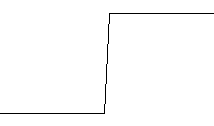
\includegraphics[scale=0.4]{Frequency/Binary}} &
\raisebox{-1.2\height}{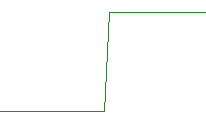
\includegraphics[scale=0.45]{Frequency/BinaryEvolved}} &  
1
\\
    \hline
   \begin{equation} f(x) = sin(2x \cdot 2\pi) \nonumber \end{equation}  &
   \raisebox{-1.2\height}{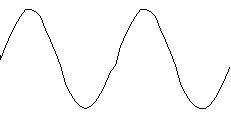
\includegraphics[scale=0.4]{Frequency/Sin1}}
       &  
       \raisebox{-1.2\height}{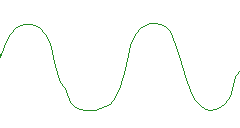
\includegraphics[scale=0.4]{Frequency/Sin1Evolved}}& 
       0.9933
\\
   \hline
   \begin{equation} f(x) = 0.2 \cdot sin(4x\cdot 2\pi+0.5) \nonumber \end{equation}  &
   \raisebox{-1.2\height}{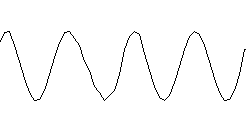
\includegraphics[scale=0.4]{Frequency/Sin2}} & 
   \raisebox{-1.2\height}{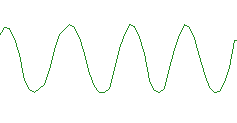
\includegraphics[scale=0.4]{Frequency/Sin2Evolved}}
   &
   0.9996  \\
   \hline
    \end{tabular}
\end{center}
As the results shows, the SUPG seems to match the functions pretty good. However a reason for the imprecision in the sine function, could be explained by the bipolar sigmoid that every output neuron is using as the activation function. This can be seen at the peaks and valleys of the sine, which are more curved.
\\
\\
However since the SUPG will be used to generate multiple frequencies (depending on their position on the substrate) it would be interesting to see how well it is at discovering multiple frequencies. The following shows how well the SUPG is at recognizing multiple functions.
\begin{center}
    \begin{tabular}{ | p{4.5cm} | l | l | l |}
    \hline
    Function & Original & Evolved & Fitness ($ F $) \\ \hline
    \begin{equation} f(x) =
    \begin{cases}
      -1, & \text{if}\ x<0.5 \\
      1, & \text{otherwise}
    \end{cases} \nonumber \end{equation}
    \begin{equation} g(x) =
    \begin{cases}
      1, & \text{if}\ x<0.5 \\
      -1, & \text{otherwise}
    \end{cases} \nonumber \end{equation} & 
    \raisebox{-1.7\height}{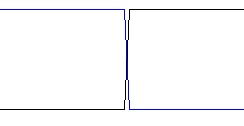
\includegraphics[scale=0.4]{Frequency/BinaryMultiple}}
     &
     \raisebox{-1.7\height}{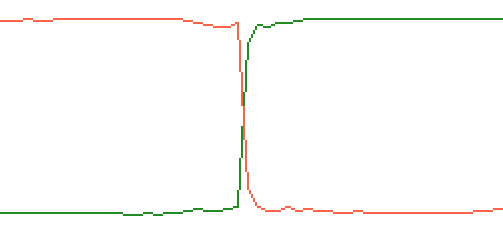
\includegraphics[scale=0.4]{Frequency/BinaryMultipleEvolved_v2}}
     &  
     0.992
     
\\
    \hline
   \begin{equation} f(x) = sin(x \cdot 2\pi) \nonumber \end{equation}  
   \begin{equation} g(x) = sin(6x \cdot 2\pi) \nonumber \end{equation}&
   \raisebox{-1.7\height}{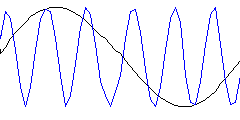
\includegraphics[scale=0.4]{Frequency/Sin1Multiple}}
       &  
       \raisebox{-1.7\height}{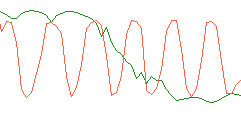
\includegraphics[scale=0.4]{Frequency/Sin1MultipleEvolved_v3}}
       & 
       0.900
\\
   \hline
    \begin{equation} f(x) =
    \begin{cases}
      -1, & \text{if}\ x<0.5 \\
      1, & \text{otherwise}
    \end{cases} \nonumber \end{equation}  
    \begin{equation} g(x) = sin(6x \cdot 2\pi) \nonumber \end{equation}
    \begin{equation} h(x) = 0.7 \cdot sin(4x \cdot 2\pi+0.5) \nonumber \end{equation}&
   \raisebox{-1.8\height}{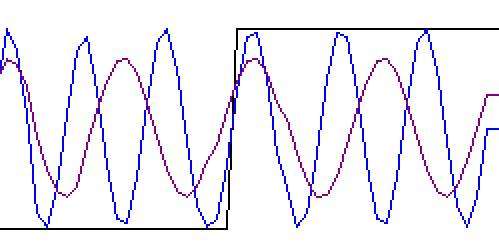
\includegraphics[scale=0.4]{Frequency/Sin3Multiple}}
 & 
 \raisebox{-1.8\height}{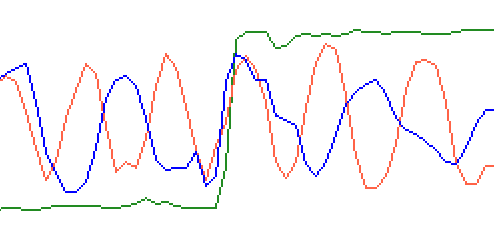
\includegraphics[scale=0.4]{Frequency/Sin3MultipleEvolved}}
   &  
   0.83
   \\
   \hline
    \end{tabular}
\end{center}
The number of generations was increased to 800, since it took more time for the results to stagnate. I also ran the evolution for each function up to five times, and only showcased the best. The reason for this, is that it sometimes will get stuck in a local optima, and wouldn't improve significantly enough. I only showed the best results, since the motivation for this experiment is to get intuition of how good the SUPG is at recognizing oscillations in the best case.
\\
\\
As can be seen from the results, the SUPG has a harder time replicating multiple functions compared to replicating single functions. However I still think the results here is pretty good, as it's still possible to tell the different frequencies apart.
\subsection{Experiment 2 - Timely split task (Prey-Predator)}
Now that I've tested how good the SUPG is at recognizing different oscillations, it's time to test how well the two new methods perform on an actual problem that requires multitasking. To do this I've come up with a simple domain that has a very clear split between two different task. The domain is inspired by pac-man and consist of two task, one where the agent is a prey and another where it is the predator. A detailed explanation of the domain and the sensors is given in the beginning of this section, and is then followed by the results of each method. 
\subsubsection{Prey-Predator Domain}
The idea with this domain is to have a relatively simple domain that has a very clear split between two tasks. The switch happens in a timely manner to ensure the agent is forced to experience both tasks - unlike a environmental task, where the agent first has to "discover" the task based on for example a position in the domain.
\\
\\
The Prey-Predator domain consist of 1 agent and 3 enemies that are placed on a square board. The board is using a wrap-around design, so if you pass one of the edges you will appear on the opposite edge. The agent and the enemies can only move in four directions: up, down, left and right. The agent moves one unit per tick, whereas the enemies only move one unit on every second tick - so the agent moves at twice the speed of an enemy.
\\
\\
The enemies have two states: edible and threat (i.e. not edible) and all agents will switch at the same time after $ x $ ticks. When enemies are edible they will move away from the agent, by going in the direction that increases the manhattan distance to the agent. If the agent catches an edible enemy, the fitness will be increase by 1 and the enemy will be spawned to a random position when next switch happens. When enemies are a threat they will move towards the agent by choosing the xy-component that is highest. If the agent touches a threat enemy, the fitness will decrease by 1 and will get spawned to a random position when next switch happens. Regardless if an enemy was hit, each switch introduces a cooldown where the enemies won't move for $ x $ ticks. This is done to give the agent a fair chance to flee from an enemy turning into a threat.
\begin{figure}[!ht]
\centering
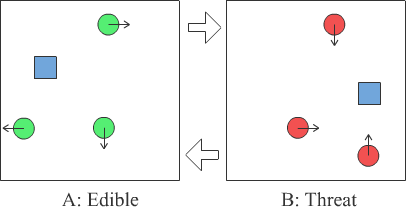
\includegraphics[scale=0.5]{PreyPredatorDomain}
\caption{}
\end{figure}
\subsubsection{Sensors}
All networks have 6 inputs and a minimum of 4 outputs. One input is used for bias. A second input is used for sensing the different task: 1 if enemies are edible and 0 otherwise. The last 4 input is used to sense where the nearest enemy in each direction is located by using the manhattan distance. The distance is clamped between 0 and 100 and divided by 100, so the input span from 0 to 1 - where 0 is close and 1 is far away. The four outputs indicate each direction, and the one output with the highest value is the direction the agent will choose.
\subsubsection{Results}
Since the random spawning position in the domain is likely to make the results noisy, I will be using a fixed seed for all of the evaluations. Each method used 65 generations, and was run for x times in total. The mean and 95\% percentile for each method are shown in the following graph.
\begin{figure}[!ht]
\centering
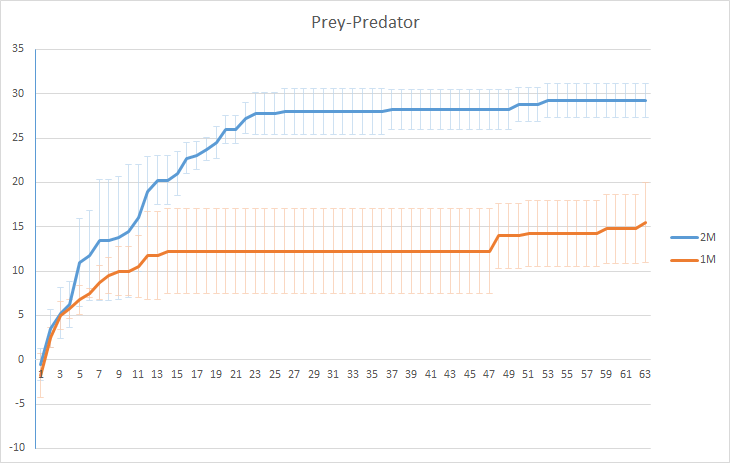
\includegraphics[scale=0.5]{Results/PreyPredatorResults}
\caption{}
\end{figure}
\\
As can be seen from the results there is a clear split between the method using two modules(2M) and the method using one method(1M). This result suggest that the domain is capable to be used as an example for multimodal behaviors. However my new methods (MiO-HyperNEAT) just don't seem to discover these new modules or at least not in a meaningful and measurable way.
\subsection{Experiment 3 - Environmental split task (Two Rooms)}
As can be seen from the results of the previous experiment, my methods didn't seem to perform very well. One of the reasons could be that the new methods just isn't that good at discovering new modules. Another reason could be that the general setup was flawed and that the previous domain wasn't a good representative for these new methods. To account for this I've decided to change the domain to something which have been used in other multitasking papers.
\\
\\
The two domains I will be using are "Dual Task" and "Two Rooms" as used in the MB-HyperNEAT paper by Schrum.
\subsubsection{Dual Task}
The dual task domain was first introduced to evaluate Evolvable-Substrate HyperNEAT[ref] and was later used to evaluate multitasking in MB-HyperNEAT[]. The dual task domain consist of two isolated task: foraging and hallway navigation.
\\
\\
In the foraging task the agent has to visit 4 way points in a specific order.
\\
\\
The hallway navigation.
\begin{figure}[!ht]
\centering
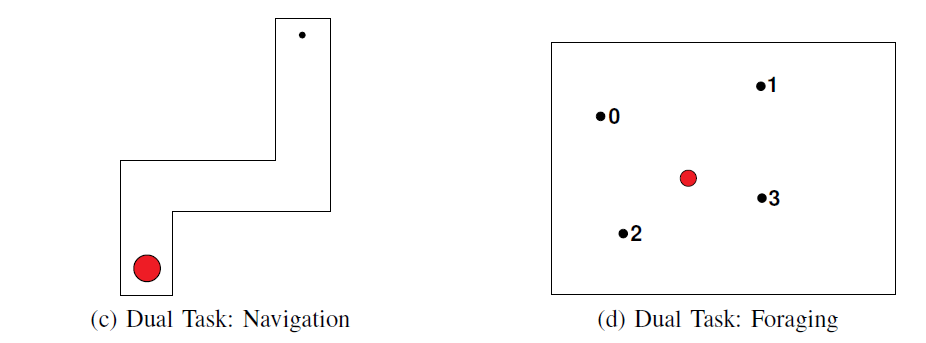
\includegraphics[scale=0.4]{DualTaskDomain}
\caption{}
\end{figure}
\subsubsection{Two Rooms}
\subsubsection{Results}
\end{document}